\documentclass[aspectratio=169]{beamer}

% Theme
\usetheme{Madrid}
\usecolortheme{dolphin}

% Packages
\usepackage[utf8]{inputenc}
\usepackage{graphicx}
\usepackage{booktabs}
\usepackage{tikz}
\usetikzlibrary{shapes.geometric, arrows, positioning}

% Remove navigation symbols
\setbeamertemplate{navigation symbols}{}

% Title information
\title{A Study of Embeddings, LLMs, and RAG Methods}
\subtitle{Information Retrieval -- Project Stage 1}
\author{Patrascu Adrian \and Modiga Miriam \and Toderian Vitalii}
\institute{Faculty of Automatic Control and Computer Science\\Politehnica University of Bucharest}
\date{November 2024}

\begin{document}

%==============================================================================
% Slide 1: Title
%==============================================================================
\begin{frame}
\titlepage
\end{frame}

%==============================================================================
% Slide 2: Project Overview
%==============================================================================
\begin{frame}{Project Overview}

\textbf{Goal}: Benchmark RAG retrieval methods for Information Retrieval

\vspace{0.5cm}

\begin{columns}
\column{0.5\textwidth}
\textbf{What we compare:}
\begin{itemize}
    \item ColBERT vs FAISS
    \item Sparse vs Dense embeddings
    \item Multiple open-source LLMs
\end{itemize}

\column{0.5\textwidth}
\textbf{Evaluation:}
\begin{itemize}
    \item 2-3 IR benchmarks
    \item Conversational tests
    \item Accuracy, speed, memory
\end{itemize}
\end{columns}

\end{frame}

%==============================================================================
% Slide 3: ColBERT
%==============================================================================
\begin{frame}{ColBERT -- Late Interaction Retrieval}

\begin{columns}
\column{0.6\textwidth}
\textbf{Key Concept}: Token-level matching

\vspace{0.3cm}

\textbf{How it works}:
\begin{enumerate}
    \item Encode query \& document with BERT
    \item Store per-token embeddings
    \item Compute MaxSim for relevance
\end{enumerate}

\vspace{0.3cm}

\textbf{Advantages}:
\begin{itemize}
    \item High accuracy
    \item Pre-computed doc embeddings
    \item Fine-grained semantic matching
\end{itemize}

\column{0.4\textwidth}
\begin{block}{MaxSim Score}
$$S_{q,d} = \sum_{i} \max_{j} E_{q_i} \cdot E_{d_j}^T$$
\end{block}

\vspace{0.3cm}

\small
\textbf{Paper}: Khattab \& Zaharia, SIGIR 2020
\end{columns}

\end{frame}

%==============================================================================
% Slide 4: FAISS
%==============================================================================
\begin{frame}{FAISS -- Similarity Search at Scale}

\begin{columns}
\column{0.5\textwidth}
\textbf{Key Concept}: Approximate nearest neighbor

\vspace{0.3cm}

\textbf{Index Types}:
\begin{itemize}
    \item \textbf{Flat}: Exact search
    \item \textbf{IVF}: Inverted file
    \item \textbf{HNSW}: Graph-based
    \item \textbf{PQ}: Compressed
\end{itemize}

\column{0.5\textwidth}
\textbf{Advantages}:
\begin{itemize}
    \item Very fast queries
    \item GPU acceleration
    \item Billion-scale support
    \item Memory efficient
\end{itemize}

\vspace{0.3cm}

\small
\textbf{Paper}: Johnson et al., 2017
\end{columns}

\end{frame}

%==============================================================================
% Slide 5: Embedders & LLMs
%==============================================================================
\begin{frame}{Embedders \& LLMs}

\begin{columns}
\column{0.5\textwidth}
\textbf{Sparse Embedders}:
\begin{itemize}
    \item BM25 (baseline)
    \item SPLADE
\end{itemize}

\vspace{0.3cm}

\textbf{Dense Embedders}:
\begin{itemize}
    \item all-MiniLM-L6-v2
    \item bge-base-en-v1.5
    \item e5-base-v2
\end{itemize}

\column{0.5\textwidth}
\textbf{Open-source LLMs}:
\begin{itemize}
    \item Llama 2 7B
    \item Mistral 7B
    \item Phi-2
    \item Zephyr 7B
\end{itemize}

\vspace{0.3cm}

\textbf{Benchmarks}:
\begin{itemize}
    \item MS MARCO
    \item Natural Questions
\end{itemize}
\end{columns}

\end{frame}

%==============================================================================
% Slide 6: Technology Stack
%==============================================================================
\begin{frame}{Technology Stack}

\begin{columns}
\column{0.5\textwidth}
\begin{table}
\small
\begin{tabular}{@{}ll@{}}
\toprule
\textbf{Component} & \textbf{Tech} \\
\midrule
Language & Python 3.10+ \\
DL Framework & PyTorch 2.0+ \\
LLMs & Transformers, vLLM \\
RAG & LangGraph \\
ColBERT & RAGatouille \\
Vectors & FAISS \\
\bottomrule
\end{tabular}
\end{table}

\column{0.5\textwidth}
\textbf{Key Libraries}:
\begin{itemize}
    \item sentence-transformers
    \item datasets (HuggingFace)
    \item ranx (evaluation)
\end{itemize}

\vspace{0.3cm}

\textbf{LangGraph}: Orchestrates conversational RAG pipeline with state management
\end{columns}

\end{frame}

%==============================================================================
% Slide 7: System Architecture
%==============================================================================
\begin{frame}{System Architecture}

\begin{center}
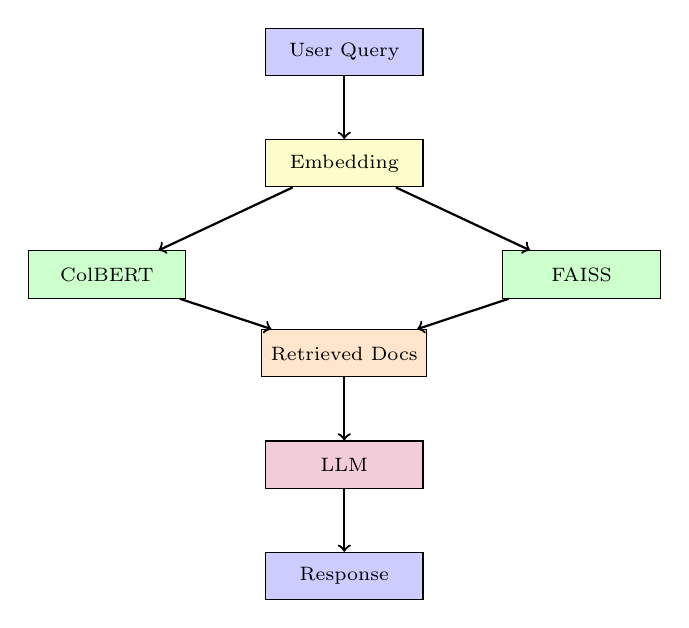
\begin{tikzpicture}[
    node distance=0.8cm,
    box/.style={rectangle, draw, minimum width=2cm, minimum height=0.6cm, align=center, font=\scriptsize},
    arrow/.style={->, thick}
]

% Nodes
\node[box, fill=blue!20] (query) {User Query};
\node[box, below=of query, fill=yellow!20] (embed) {Embedding};
\node[box, below left=0.8cm and 1cm of embed, fill=green!20] (colbert) {ColBERT};
\node[box, below right=0.8cm and 1cm of embed, fill=green!20] (faiss) {FAISS};
\node[box, below=1.8cm of embed, fill=orange!20] (docs) {Retrieved Docs};
\node[box, below=of docs, fill=purple!20] (llm) {LLM};
\node[box, below=of llm, fill=blue!20] (response) {Response};

% Arrows
\draw[arrow] (query) -- (embed);
\draw[arrow] (embed) -- (colbert);
\draw[arrow] (embed) -- (faiss);
\draw[arrow] (colbert) -- (docs);
\draw[arrow] (faiss) -- (docs);
\draw[arrow] (docs) -- (llm);
\draw[arrow] (llm) -- (response);

\end{tikzpicture}
\end{center}

\end{frame}

%==============================================================================
% Slide 8: Evaluation Metrics
%==============================================================================
\begin{frame}{Evaluation Metrics}

\begin{columns}
\column{0.5\textwidth}
\textbf{Retrieval Metrics}:
\begin{itemize}
    \item MRR@k (Mean Reciprocal Rank)
    \item Recall@k
    \item NDCG@k
\end{itemize}

\vspace{0.3cm}

\textbf{Generation Metrics}:
\begin{itemize}
    \item BLEU, ROUGE-L
    \item BERTScore
\end{itemize}

\column{0.5\textwidth}
\textbf{Efficiency Metrics}:
\begin{itemize}
    \item Query latency (ms)
    \item Index size (GB)
    \item Memory usage
    \item Throughput (QPS)
\end{itemize}
\end{columns}

\end{frame}

%==============================================================================
% Slide 9: Challenges
%==============================================================================
\begin{frame}{Potential Challenges}

\begin{columns}
\column{0.5\textwidth}
\textbf{Technical}:
\begin{itemize}
    \item Memory constraints (ColBERT indexes are large)
    \item GPU requirements for LLMs
    \item Indexing time differences
\end{itemize}

\column{0.5\textwidth}
\textbf{Methodological}:
\begin{itemize}
    \item Hyperparameter tuning
    \item Fair comparison setup
    \item LLM prompt consistency
\end{itemize}
\end{columns}

\vspace{0.5cm}

\begin{table}
\centering
\small
\begin{tabular}{@{}lcc@{}}
\toprule
\textbf{Aspect} & \textbf{ColBERT} & \textbf{FAISS} \\
\midrule
Accuracy & Higher & Lower \\
Speed & Slower & Faster \\
Index Size & Larger & Smaller \\
\bottomrule
\end{tabular}
\end{table}

\end{frame}

%==============================================================================
% Slide 10: Timeline & Questions
%==============================================================================
\begin{frame}{Timeline \& Questions}

\textbf{Project Stages}:
\begin{enumerate}
    \item \textbf{Stage 1} (Current): Project description, architecture
    \item \textbf{Stage 2}: Implementation of retrieval pipelines
    \item \textbf{Stage 3}: Benchmark evaluation
    \item \textbf{Final}: Report with findings
\end{enumerate}

\vspace{0.5cm}

\begin{center}
\Large
\textbf{Questions?}

\vspace{0.3cm}

\normalsize
Thank you for your attention!
\end{center}

\end{frame}

\end{document}
